\documentclass[paper=a4, parskip=half-]{scrartcl}
\usepackage[utf8]{inputenc}

\usepackage{amsmath}
\usepackage{mathtools}
\usepackage{marvosym} % for the \Lightning symbol
\usepackage{amssymb} % more icons/symbols
\usepackage{tablefootnote} % for footnotes in tables
% not in standard texlive, can't be asked to figure it out now
%\usepackage{ccicons} % creative commons icon
\usepackage{hyperref} % for hyper links
\usepackage[dvipsnames]{xcolor} % to color stuff -- dvipnames for additional color names
\usepackage[shortlabels]{enumitem} % to modify enumeration labels
\usepackage{tcolorbox} % for colored boxes - see https://tex.stackexchange.com/questions/66154/how-to-construct-a-coloured-box-with-rounded-corners/172608#172608
\usepackage{tikz} % drawing stuff
\usepackage{eurosym} % € (no, default LaTeX font doesn't include it)
\usepackage{natbib}
\usepackage{graphicx}

\usepackage{geometry}
 \geometry{
 a4paper,
 left=20mm,
 right=20mm,
 top=20mm,
 bottom=30mm,
 }


\title{Security of Wireless Networks}
\author{\texttt{\{thgoebel\}@ethz.ch}}
\date{ETH Zürich, HS 2020}

% Custom commands
\newcommand{\setzeroone}{\lbrace 0, 1 \rbrace} % => {0,1} (Notice the missing $$)
\newcommand{\horizontaldivider}{\begin{center} \line(1,0){350} \end{center}}

\begin{document}

\begin{titlepage}
\maketitle
\vspace{5cm}
\thispagestyle{empty}


\begin{abstract}
This documents is a summary for the course \textit{Security of Wirless Networks (SOWN)} at ETH Zurich.

This summary is created during the autumn semester 2020.
But due to the few changes in syllabus content in the past we have reason to believe that it is also relevant beyond that very semester.

We do not guarantee correctness or completeness, nor is this document endorsed by the lecturers.
Feel free to point out any erratas.
\end{abstract}

\end{titlepage}

\tableofcontents
%\listoffigures
%\listoftables
\newpage


\section{Wireless Basics}

\begin{figure}[h]
	\centering
	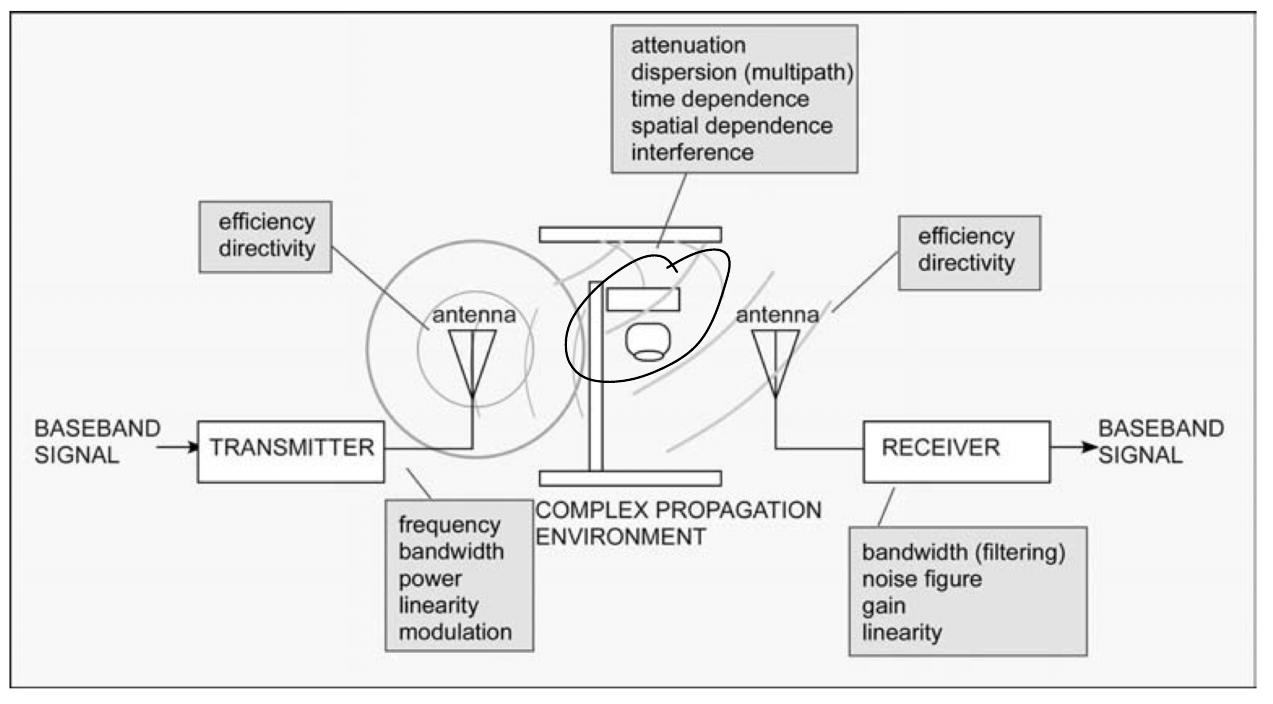
\includegraphics[scale=0.4]{images/1-wireless-system.png}
	\caption{A wireless system, its basic components and characteristic measures}%
	\label{fig:wireless-system}
\end{figure}

\paragraph{Radio Frequency Signal}
Electromagnetic radiation, with waves being created in the antenna by an
alternating current at the desired frequency. Mathematically described as a
function of the time $t$:
\[ v(t) = A \sin (2 \pi f t + \phi) \]
with amplitude $A$, frequency $f$ and phase $\phi$. Also recall that the period
is $T = \frac{1}{f}$ and the wavelength (distance traveled during one period)
is $\lambda = \frac{v}{f}$ (usually $v=c$ speed of light).

\paragraph{Bandwidth}
The capacity of a communications link to transmit the maximum amount of data
from one point to another over a connection in a given amount of time (in bits
per second bps). An analogy: The amount of water that can flow through a water
pipe.

In other words, the measure of frequency content of the signal. E.g.\ the human
voice contains frequencies in the range from 30 Hz to 10 kHz, and the bandwidth
of a single 802.11 channel is 22 MHz.

Note that often the bandwidth of the base-band and that of the carrier (and
thus that of the modulated signal) differ! E.g.\ see spread spectrum techniques
(\autoref{sec:jamming-resistant-comm}). Low variability of the signal in time
corresponds to a small bandwidth, whereas a high variability corresponds to a
large bandwidth

\begin{figure}[h]
	\centering
	
\includegraphics[scale=0.35]{images/1-wifi-channels.png}
	\caption{2.4 GHz WiFi Channels \href{https://en.wikipedia.org/wiki/List\_of\_WLAN\_channels\#/media/File:2.4\_GHz\_Wi-Fi\_channels\_(802.11b,g_WLAN).svg}{[Source]}}%
	\label{fig:wifi-channels}
\end{figure}

\paragraph{Baseband}
An original transmission signal that has not been modulated or has been
demodulated to its original frequency, aka the actual \textbf{information
	signal}. Most telecommunication protocols require base-band signals to be
converted, or modulated, to a higher frequency in order to be transmitted over
long distances.

\paragraph{Carrier}
A transmitted electromagnetic pulse or wave at a steady base frequency of
alternation on which information can be imposed. Typically \textbf{a pure
	sinusoid of a particular frequency and phase} that will carry the information.
Usually the frequency of the carrier is much higher than that of the baseband.
To go from baseband to passband, we need to multiply the analytic signal with a
carrier, where $f_c$ is the carrier frequency and $a(t)$ is the amplitude.
\[ x_{RF} (t) = \Re \{a(t)e^{i\theta (t)}\} = a(t) \cos (2 \pi f_c t + \theta(t))\]

\subparagraph{Upconversion}
This process is called \textbf{up-conversion}, and it's necessary mainly for
two reasons: to enable simultaneous transmission of different signals by using
a different carrier frequency (for each transmission) and to transform a
complex signal into a real one, since only real signals can actually be
transmitted. At the receiver, it's then down-converted such that the subsequent
processing can be done in the complex-valued baseband domain.

In order to actually perform the up-conversion, we need an oscillator to
produce the cosine wave at the chosen (carrier) frequency and a mixer to
multiply it with the baseband signal, producing the frequency shift.

\paragraph{Modulated Signal}
A carrier that has been loaded or modulated with the information signal.

\paragraph{Modulation}
Process of imposing the baseband onto the carrier. The baseband is used to
alter one aspect of the carrier, such as: signal strength (\textit{amplitude
	modulation AM}), frequency (\textit{frequency modulation FM}), phase
(\textit{phase modulation PM}). In other words, one of the values $A, f, \phi$
in the above equation of the signal is manipulated.

\paragraph{Amplitude-shift keying ASK}
Modulation technique varying the amplitude of the signal.

\paragraph{Frequency-shift keying FSK}
Modulation technique varying the frequency of the carrier.

\paragraph{Phase-shift keying PSK}
Modulation technique varying the phase of the carrier. It's used, for example,
in WiFi, RFID, Bluetooth. Specific versions include Binary PSK, Quadrature PSK
and Differential PSK.\@ Example: if the baseband bit is 0 do nothing to the
carrier, if it is 1 shift the carrier phase by $\pi$.

\paragraph{On-Off-Keying OOK}
Simple form of amplitude-shift keying ASK.\@ Represents data as the presence
(1) or absence (0) of a signal. E.g.\ Morse code.

\paragraph{I-Q Signal Representation}
A pair of periodic signals are said to be in `quadrature' when they differ in
phase by 90 degrees (e.g.\ the sine and cosine wave). The `in-phase' or
reference signal is referred to as `I' (conventionally cosine), and the signal
that is shifted by 90 degrees (in quadrature) is called `Q' (conventionally
sine). It's used to represent modulations.
\[ I(t) = a(t) \cos (\phi(t)) \leftarrow  \textrm{Analytic signal, } a(t) \textrm{ is the amplitude}\]
\[ Q(t) = a(t) \sin (\phi(t)) \]

\paragraph{Antenna}
Interface between radio waves in the air and electric alternating currents in a
conductor. Types include: omni/dipole, yagi, horn, can-tenna.

The directionality of an antenna described how well it transmits/receives into
a particular direction.
\begin{itemize}
	\item \textbf{isotropic} --- Theoretical, radiates with the same intensity equally in all directions. Often used as a reference antenna when calculating the gain.
	\item \textbf{omnidirectional} --- Radiates equally well in all directions in a flat horizontal plane. Most common types in consumer devices.
	\item \textbf{directional} --- Radiates best in a given direction by focussing its power. Can thus work with weaker signals than an omnidirectional antenna of the same power.
\end{itemize}

\begin{figure}[h]
	\centering
	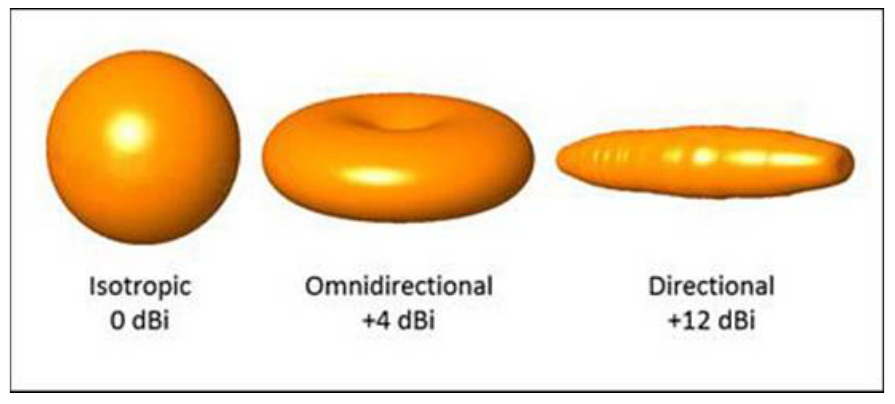
\includegraphics[scale=0.4]{images/1-directionality.png}
	\caption{Antenna directionality}%
	\label{fig:directionality}
\end{figure}

\paragraph{Phased Array}
Array of fixed antennas where the phase of each signal is dynamically adjusted
so that the signal will be in phase when viewed from a given direction. Allows
\textit{beam steering} towards a specific direction. Possible applications? Can
it be used to achieve security (e.g.\ confidentiality)?

\begin{figure}[h]
	\centering
	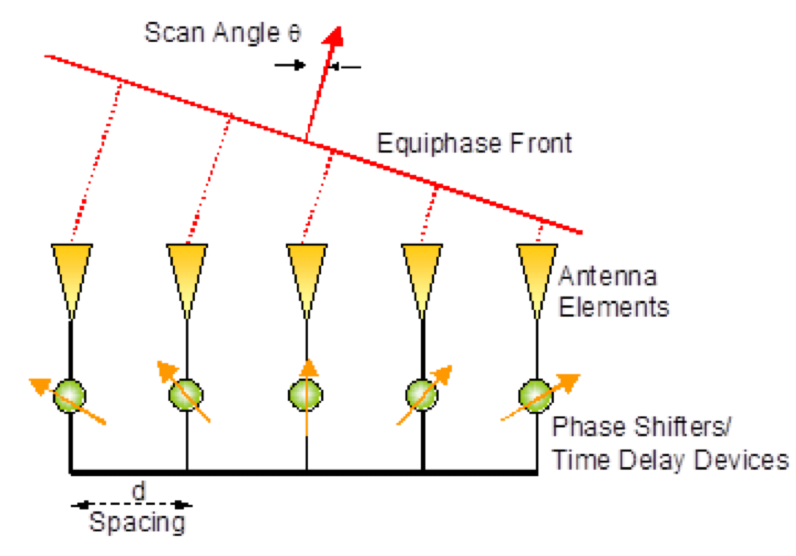
\includegraphics[scale=0.4]{images/1-beam-steering.png}
	\caption{Beam steering}%
	\label{fig:beam-steering}
\end{figure}

\paragraph{Transmitter/Receiver}
Converts from digital to analogue, applies modulation and connects to the
antenna (and vice versa). Properties: transmitted power, carrier frequency,
information bandwidth, modulation type, receiver sensitivity.

\paragraph{Software Defined Radio SDR}
Flexible, low-cost transmitter/receiver. Implements components (mixer,
amplifier, de-/modulator) in software rather than processing the signal in
hardware.

\paragraph{Channel equation}
See \autoref{fig:signal-strength}.

signal strength at the receiver $=$ transm.\ power $+$ transm.\ antenna gain
$-$ link loss $+$ receiv.\ antenna gain

Note that, in free space, the power density of an EM wave obeys the
inverse-square law:
\[p \propto \frac{1}{d^2} \]

\begin{figure}[h]
	\centering
	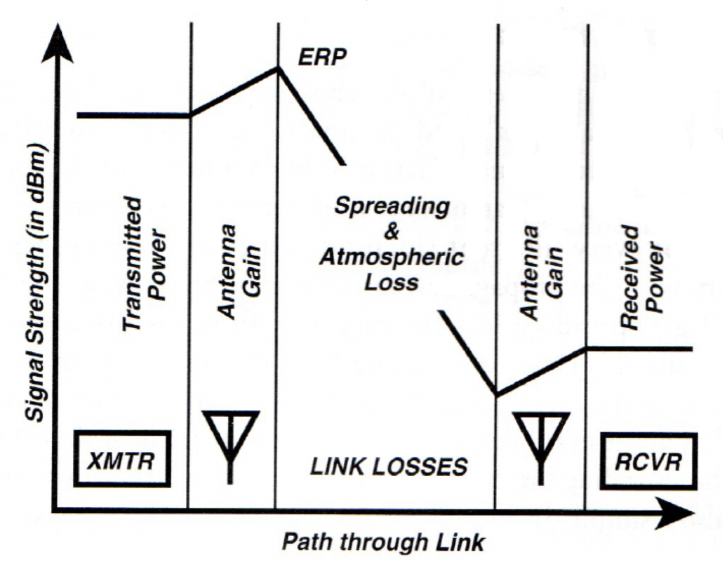
\includegraphics[scale=0.4]{images/1-signal-strength.png}
	\caption{Signal strength across the channel (ERP = Effective Radiated Power)}%
	\label{fig:signal-strength}
\end{figure}

\paragraph{Receiver sensitivity}
The weakest signal from which the receiver can still obtain the desired
information signal. Depends not just on the antenna gain, but also on other
factors such as the noise.

\paragraph{Decibel}
\begin{itemize}
	\item dBm --- signal strength in dB / 1 milliwatt mW
	\item dBW --- signal strength in dB / 1 watt W
	\item dBi --- antenna gain in dB / antenna gain of isotopic antenna in dB
\end{itemize}
Calculating a value in dB \[ dB(n) = 10 \log_{10} (n) \quad \text{ and } \quad dBm(n) = 10 \log_{10} (n / 1 mW) \]

\paragraph{Power Spectral Density diagram}
Depicts the power density (in dB) for a range of frequencies. In simple terms,
it shows how strong the signal is at a given frequency.

For a signal $x_T(t)$ defined between $(-\frac{T}{2}, \frac{T}{2})$, its power
in the time domain will be \[P = \lim_{T\rightarrow \infty} \frac{1}{T} \int |x_T(t)|^2 dt \] and its power in the frequency domain will be \[PSD(f) = \lim_{T\rightarrow \infty} \frac{1}{T} \int |X_T(f)|^2 df \]

\paragraph{Security Goals}
Reasons: \textit{security} (integrity, confidentiality, authentication),
\textit{regulatory} (personal liability for misuse of one's network access),
\textit{safety} (RF-enabled implants).

Just reducing transmission power, hoping that the attacker will be too far away
to listen on / send / modify messages, is NOT a solution. In fact, WiFi signals
can be received 10 km away, and similarly Bluetooth at 1 km distance (with
good, directed equipment).

Example: \textit{Passive Keyless Entry and Start systems (PKES)}, i.e.\
wireless car keys. Wrongly assume communication implies physical proximity
(relay attack). Needs: Authenticated proximity verification, message
authentication.

\subsection{Questions}
\textbf{Does a wireless channel, in general, affect all frequencies of a signal equally?} It depends on what kind of noise/interference is present on the channel. If it's general thermal noise, then yes, all frequencies will be generally affected in a similar way. However, if there are other communications happening, then the frequencies used by those transmissions will have a greater noise level.
Also, higher frequency signals suffer from greater attenuation due to the distance traveled compared to lower frequency signals.

\textbf{Which two properties of the wireless channel are leveraged by systems that rely on those for physical-layer based key establishment?} Channel impulse response and received signal strength.

\textbf{Describe the effect of increasing or decreasing the sub-carrier spacing in an OFDM modulated signal. Assuming the overall bandwidth of the channel stays the same, how does the sub-carrier spacing affect Symbol length, Throughput and complexity of the receiver?} TODO % TODO: increasing sub carrier spacing decreases symbol length because it increases symbol time ???
% TODO: A longer symbol length makes it more resilient against multi-path interference, but it probably needs a more complex receiver.
% TODO: Throughput should stay the same ????
\newpage

\section{Jamming Basics}

\paragraph{Jamming}
Entirely preventing or reducing the ability of communicating parties to pass information, either intentionally or unintentionally.

The jamming signal needs to have the same frequency as the modulated signal.
If the latter is unknown to the attacker, they thus need to jam a wide bandwidth of frequencies to be successful.

Effectively, jamming is always a power play.

\paragraph{Symbol}
Carries one or more bit of information, depending on the modulation scheme.

\paragraph{Symbol Jamming}
Corrupts symbols such that the receiver can EITHER no interpret them OR interprets them incorrectly.\\
Targeted, low-power jamming of specific symbols is hard!

\paragraph{Communication Jamming}
Corrupts enough bits that the information cannot be reconstructed any more, despite error correction.

\paragraph{Jamming-to-Signal Ratio J/S} = $J -  S$, i.e. the difference between the jamming signal and the modulated signal in dB.
A ratio $\geq 0$ usually results in successful jamming.

\paragraph{Burn-through range}
Range in which communication still succeeds, despite jamming.

\paragraph{Attacker model} \mbox{} \\
% taken from the following chapter/deck of slides
Types: responsive, sweep, random \\
Actions: jam, insert, modify (= overshadow) \\
Power to jam/insert/modify: $P_j, P_t, P_o$ \\
\# channels to jam/insert/modify: $c_j, c_t, c_o$ \\
Total strength/power $P_T$ \\
$$ c_j P_j + c_t P_t + c_o P_o \leq P_T$$

\subsection{Jamming Resistant Communication}

\paragraph{Basic principle}
If you cannot fight (i.e. have too little power), RUN, HIDE or WAIT.
And get ad advantage over the attacker: use a shared secret.

\paragraph{Frequency Hopping Spread Spectrum FHSS}
Regularly change transmission frequency.
The pseudorandom frequency sequence is derived from a shared secret.
Sender and receiver \textbf{must} be synchronised.

Note that frequency hoppers can be detected and located, simply by looking over time from which direction someone is sending on changing frequencies.

Possible attacks:
\begin{itemize}
	\item \textbf{Partial band jammer:}
	Distribute jamming power over a subset of all hopping frequencies to achieve $J/S=0$ at least on that range.
	\item \textbf{Follower jammer:}
	Detects on which frequency communication occurs and then jams it.
	Can be protected against by using error codes (since only the final bits will be corrupted).
\end{itemize}

\paragraph{Direct Sequence Spread Spectrum DSSS}
Spreads the baseband over a larger bandwidth using a shared secret (narrowband to broadband). \\
Since the transmission power remains the same, the power density at any given frequency decreases.
Thus the spread signal can effectively ``hide under the noise'' (\autoref{fig:dsss-psd}).

To spread over more frequencies, we need a higher symbol/bit rate.
To achieve this the information signal is multiplied with a high-frequency pseudorandom sequence called \textbf{chips} or \textbf{spreading code}.
The result resembles \textbf{white noise}.
See \autoref{fig:dsss}.

During de-spreading, the signal is again multiplied with the same spreading code.
De-spreading thus converts the wideband signal into a narrowband one (this works due to the autocorrelation properties of the spreading code).
At the same time, any narrowband interference is spread out.
\\
Thus DSSS is more robust against (un)intentional interference and multipath effects, and narrowband jamming requires much more power.
Broadband jamming is possible, but inherently requires much power.

Detecting DSSS signals is difficult, but not impossible (energy detection of strong signals, signal characteristics such as constant chip rate).
Interception and modification is hard.

Example usages: GPS, 802.11b WiFi, CDMA (used in 3G).
Non-military applications mainly use DSSS for interference-resistance and use public spreading codes.
They are thus still vulnerable to malicious jamming as DoS.

\begin{figure}
	\centering
	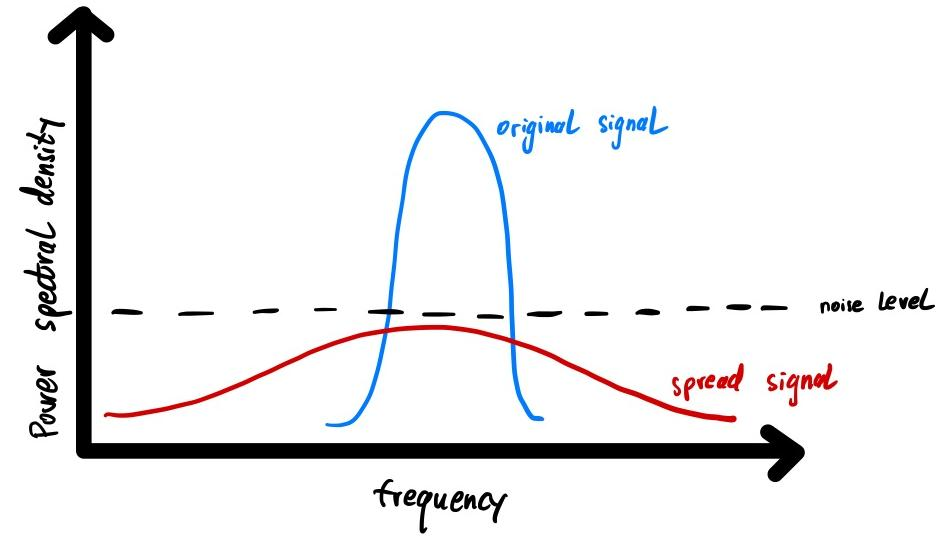
\includegraphics[scale=0.4]{images/2-dsss-psd.jpg}
	\caption{DSSS -- hiding under the noise}
	\label{fig:dsss-psd}
\end{figure}

\begin{figure}
	\centering
	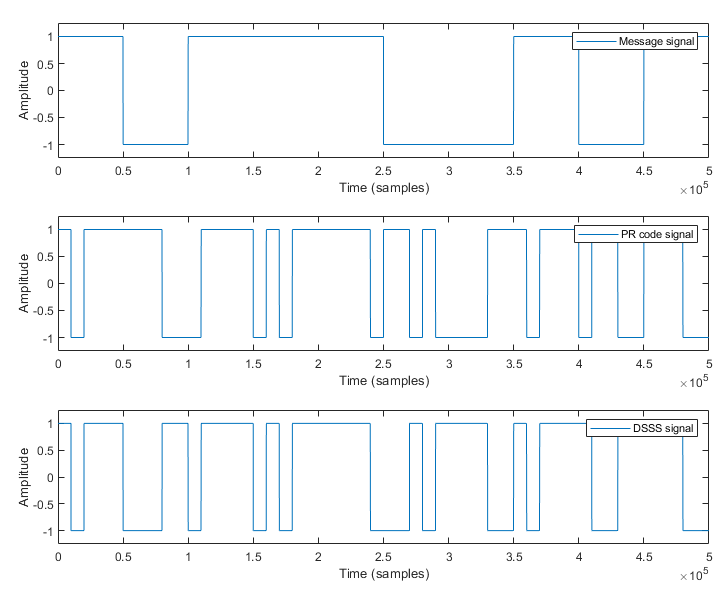
\includegraphics[scale=0.6]{images/2-dsss.png}
	\caption{DSSS -- baseband signal, spreading code, spread signal (top to bottom)}
	\label{fig:dsss}
\end{figure}

\paragraph{Processing Gain PG}
Ratio of the spread bandwidth to the baseband bandwidth, in dB.


\paragraph{Chirp Signal / Sweep Signal}
Signal in which the frequency increases and decreases over time (``sweeping'' over a bandwidth much wider than the baseband bandwidth).
Narrowband and partial-band jamming are prevented, follower jamming not so much

\paragraph{Code-Division Multiple Access CDMA}
Multiple transmitters sending in the same area simultaneously, but using different spreading codes.
Allows sharing of the same frequencies/bandwidth without interference.

\newpage

%
% Appendix
%
\appendix

%\part{Appendix}

\section{Imprint}

This document closely follows the lecture slides of the \textit{Security of Wireless Networks} lecture in the autumn semester 2020 at ETH Zurich.
Our contribution to this is editing the whole lot and refactoring even more so that it may fit the "lecture summary" style.
However, basically all graphics are copy \& pasted from the slides. If you don't want yours here, please contact us and we will remove them.

In addition, this summary is based on a summary by Sarah Kamp.

Otherwise, our part of the work is published as CC BY-NC-SA.

%\begin{center}
%\ccbyncsa
%\end{center}


%\bibliographystyle{plain}
%\bibliography{references}

\end{document}